%% fig_charactergrid.tex   (generated by make_core.py; do not edit by hand)
%% The K^x-grading of H^*(A,C) at n = 3 on the grid of pairs (r,s); the summands of H^{2n} at their true dimensions, summing to 924.
\documentclass[tikz,border=8pt]{standalone}
\usepackage{amsmath,amssymb}
\usetikzlibrary{arrows.meta,calc,decorations.pathreplacing}
%% palette.tex -- shared colour definitions for the figures
\definecolor{PInk}{RGB}{26,32,44}
\definecolor{PBlue}{RGB}{37,82,139}
\definecolor{PTeal}{RGB}{23,127,125}
\definecolor{POchre}{RGB}{193,138,44}
\definecolor{PClay}{RGB}{178,74,58}
\definecolor{PSlate}{RGB}{108,122,137}
\definecolor{PViolet}{RGB}{110,86,150}
\definecolor{WBlue}{RGB}{223,234,246}
\definecolor{WTeal}{RGB}{220,238,236}
\definecolor{WOchre}{RGB}{250,240,218}
\definecolor{WClay}{RGB}{247,229,224}
\definecolor{WSlate}{RGB}{238,241,244}
\definecolor{PMag}{RGB}{158,58,110}
\definecolor{PGrass}{RGB}{62,124,66}
\definecolor{PAmber}{RGB}{214,112,38}
\definecolor{PIndigo}{RGB}{58,64,140}
\definecolor{PRule}{RGB}{176,186,197}

%% shared macros so the standalone figures match the paper
\providecommand{\QQ}{\mathbb{Q}}
\providecommand{\ZZ}{\mathbb{Z}}
\providecommand{\RR}{\mathbb{R}}
\providecommand{\CC}{\mathbb{C}}
\providecommand{\PP}{\mathbb{P}}
\providecommand{\Kx}{K^{\times}}
\providecommand{\HW}{W}
\providecommand{\Nm}{\mathrm{N}}
\providecommand{\Hdg}{\mathrm{Hdg}}
\providecommand{\NS}{\mathrm{NS}}
\providecommand{\cA}{\mathcal{A}}
\providecommand{\cD}{\mathcal{D}}
\providecommand{\cF}{\mathcal{F}}
\providecommand{\cP}{\mathcal{P}}
\providecommand{\cO}{\mathcal{O}}
\providecommand{\cQ}{\mathcal{Q}}
\providecommand{\bbar}[1]{\overline{#1}}
\providecommand{\ch}{\operatorname{ch}}
\providecommand{\End}{\mathrm{End}}
\providecommand{\Ext}{\operatorname{Ext}}
\providecommand{\Supp}{\operatorname{Supp}}

\begin{document}
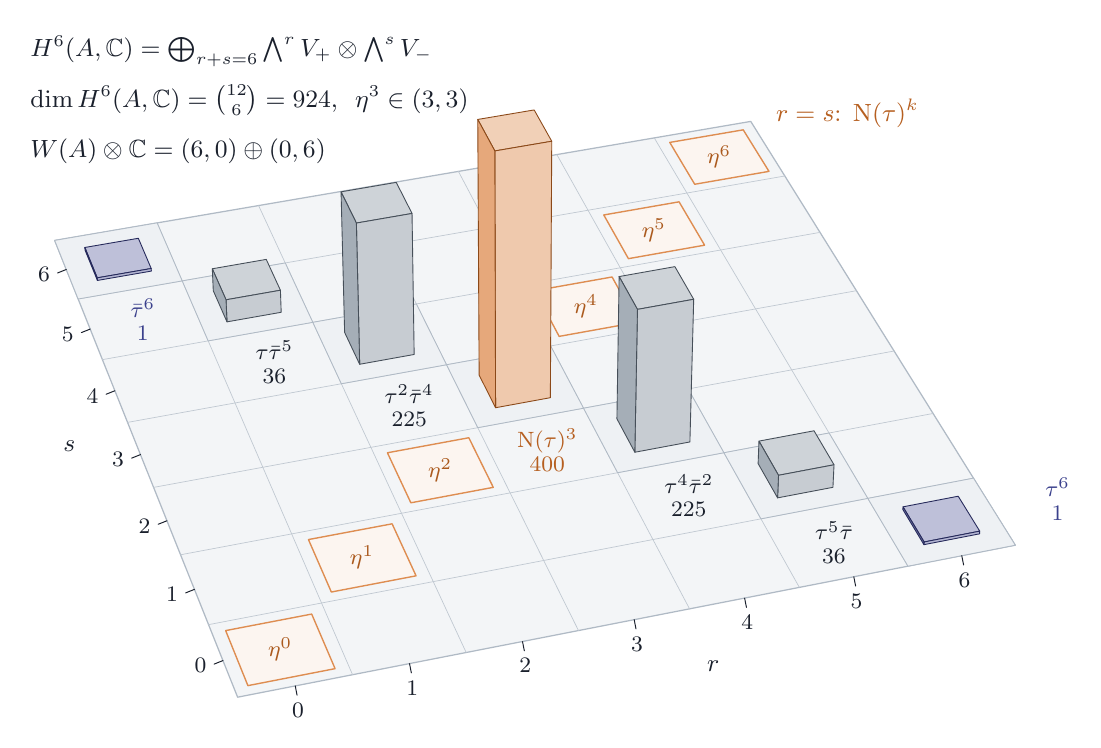
\begin{tikzpicture}[x=1cm,y=1cm,line join=round,line cap=round,
  font=\small,text=PInk,lbl/.style={inner sep=1pt}]
  \path[fill=WSlate!70,draw=PRule,line width=0.45pt] (-3.5181,-4.6240) -- (6.3586,-2.6935) -- (2.9986,2.6884) -- (-5.8414,1.1768) -- cycle;
  \draw[PRule!80,line width=0.25pt] (-2.0583,-4.3386) -- (-4.5400,1.3994);
  \draw[PRule!80,line width=0.25pt] (-3.8870,-3.7028) -- (5.8270,-1.8421);
  \draw[PRule!80,line width=0.25pt] (-0.6153,-4.0566) -- (-3.2518,1.6197);
  \draw[PRule!80,line width=0.25pt] (-4.2425,-2.8153) -- (5.3142,-1.0207);
  \draw[PRule!80,line width=0.25pt] (0.8112,-3.7778) -- (-1.9765,1.8377);
  \draw[PRule!80,line width=0.25pt] (-4.5852,-1.9596) -- (4.8191,-0.2276);
  \draw[PRule!80,line width=0.25pt] (2.2216,-3.5021) -- (-0.7140,2.0536);
  \draw[PRule!80,line width=0.25pt] (-4.9159,-1.1340) -- (4.3408,0.5385);
  \draw[PRule!80,line width=0.25pt] (3.6161,-3.2295) -- (0.5358,2.2673);
  \draw[PRule!80,line width=0.25pt] (-5.2351,-0.3371) -- (3.8784,1.2791);
  \draw[PRule!80,line width=0.25pt] (4.9950,-2.9600) -- (1.7733,2.4789);
  \draw[PRule!80,line width=0.25pt] (-5.5434,0.4328) -- (3.4313,1.9953);
  \path[fill=WSlate,draw=PRule,line width=0.30pt] (-5.5434,0.4328) -- (-4.2215,0.6629) -- (-4.5400,1.3994) -- (-5.8414,1.1768) -- cycle;
  \path[fill=WSlate,draw=PRule,line width=0.30pt] (-3.8920,-0.0989) -- (-2.5630,0.1368) -- (-2.9132,0.8907) -- (-4.2215,0.6629) -- cycle;
  \path[fill=WSlate,draw=PRule,line width=0.30pt] (-2.2007,-0.6434) -- (-0.8646,-0.4020) -- (-1.2479,0.3700) -- (-2.5630,0.1368) -- cycle;
  \path[fill=WSlate,draw=PRule,line width=0.30pt] (-0.4678,-1.2013) -- (0.8752,-0.9539) -- (0.4573,-0.1632) -- (-0.8646,-0.4020) -- cycle;
  \path[fill=WSlate,draw=PRule,line width=0.30pt] (1.3079,-1.7730) -- (2.6579,-1.5195) -- (2.2038,-0.7092) -- (0.8752,-0.9539) -- cycle;
  \path[fill=WSlate,draw=PRule,line width=0.30pt] (3.1283,-2.3590) -- (4.4851,-2.0992) -- (3.9932,-1.2687) -- (2.6579,-1.5195) -- cycle;
  \path[fill=WSlate,draw=PRule,line width=0.30pt] (4.9950,-2.9600) -- (6.3586,-2.6935) -- (5.8270,-1.8421) -- (4.4851,-2.0992) -- cycle;
  \path[fill=PAmber!7,draw=PAmber!80,line width=0.50pt] (-3.3874,-4.4773) -- (-2.2803,-4.2615) -- (-2.5774,-3.5684) -- (-3.6701,-3.7782) -- cycle;
  \path[fill=PAmber!7,draw=PAmber!80,line width=0.50pt] (-2.3278,-3.2883) -- (-1.2517,-3.0827) -- (-1.5560,-2.4223) -- (-2.6184,-2.6222) -- cycle;
  \path[fill=PAmber!7,draw=PAmber!80,line width=0.50pt] (-1.3180,-2.1552) -- (-0.2714,-1.9591) -- (-0.5817,-1.3291) -- (-1.6155,-1.5199) -- cycle;
  \path[fill=PAmber!7,draw=PAmber!80,line width=0.50pt] (0.5655,-0.0417) -- (1.5578,0.1372) -- (1.2376,0.7125) -- (0.2569,0.5382) -- cycle;
  \path[fill=PAmber!7,draw=PAmber!80,line width=0.50pt] (1.4452,0.9454) -- (2.4124,1.1165) -- (2.0884,1.6671) -- (1.1322,1.5002) -- cycle;
  \path[fill=PAmber!7,draw=PAmber!80,line width=0.50pt] (2.2871,1.8901) -- (3.2303,2.0539) -- (2.9031,2.5813) -- (1.9703,2.4215) -- cycle;
  \path[fill=PIndigo!33!white,draw=PIndigo!65!black,line width=0.32pt] (-5.3006,0.7017) -- (-4.6155,0.8204) -- (-4.7787,1.2041) -- (-5.4582,1.0875) -- cycle;
  \path[fill=PIndigo!38!white,draw=PIndigo!65!black,line width=0.32pt] (-5.2986,0.6686) -- (-4.6138,0.7874) -- (-4.6155,0.8204) -- (-5.3006,0.7017) -- cycle;
  \path[fill=PIndigo!61!white,draw=PIndigo!65!black,line width=0.32pt] (-5.2986,0.6686) -- (-5.4561,1.0546) -- (-5.4582,1.0875) -- (-5.3006,0.7017) -- cycle;
  \path[fill=PSlate!33!white,draw=PSlate!65!black,line width=0.32pt] (-3.6651,0.4230) -- (-2.9744,0.5442) -- (-3.1544,0.9360) -- (-3.8395,0.8169) -- cycle;
  \path[fill=PSlate!38!white,draw=PSlate!65!black,line width=0.32pt] (-3.6531,0.1427) -- (-2.9647,0.2642) -- (-2.9744,0.5442) -- (-3.6651,0.4230) -- cycle;
  \path[fill=PSlate!61!white,draw=PSlate!65!black,line width=0.32pt] (-3.6531,0.1427) -- (-3.8270,0.5378) -- (-3.8395,0.8169) -- (-3.6651,0.4230) -- cycle;
  \path[fill=PSlate!33!white,draw=PSlate!65!black,line width=0.32pt] (-2.0097,1.3974) -- (-1.3029,1.5194) -- (-1.5035,1.9140) -- (-2.2044,1.7941) -- cycle;
  \path[fill=PSlate!38!white,draw=PSlate!65!black,line width=0.32pt] (-1.9681,-0.3960) -- (-1.2760,-0.2715) -- (-1.3029,1.5194) -- (-2.0097,1.3974) -- cycle;
  \path[fill=PSlate!61!white,draw=PSlate!65!black,line width=0.32pt] (-1.9681,-0.3960) -- (-2.1591,0.0087) -- (-2.2044,1.7941) -- (-2.0097,1.3974) -- cycle;
  \path[fill=PAmber!33!white,draw=PAmber!65!black,line width=0.32pt] (-0.2513,2.3134) -- (0.4713,2.4365) -- (0.2482,2.8340) -- (-0.4682,2.7133) -- cycle;
  \path[fill=PAmber!38!white,draw=PAmber!65!black,line width=0.32pt] (-0.2419,-0.9478) -- (0.4538,-0.8203) -- (0.4713,2.4365) -- (-0.2513,2.3134) -- cycle;
  \path[fill=PAmber!61!white,draw=PAmber!65!black,line width=0.32pt] (-0.2419,-0.9478) -- (-0.4509,-0.5333) -- (-0.4682,2.7133) -- (-0.2513,2.3134) -- cycle;
  \path[fill=PSlate!33!white,draw=PSlate!65!black,line width=0.32pt] (1.5599,0.3011) -- (2.2742,0.4294) -- (2.0353,0.8440) -- (1.3270,0.7181) -- cycle;
  \path[fill=PSlate!38!white,draw=PSlate!65!black,line width=0.32pt] (1.5267,-1.5132) -- (2.2260,-1.3825) -- (2.2742,0.4294) -- (1.5599,0.3011) -- cycle;
  \path[fill=PSlate!61!white,draw=PSlate!65!black,line width=0.32pt] (1.5267,-1.5132) -- (1.2990,-1.0884) -- (1.3270,0.7181) -- (1.5599,0.3011) -- cycle;
  \path[fill=PSlate!33!white,draw=PSlate!65!black,line width=0.32pt] (3.3511,-1.8060) -- (4.0563,-1.6724) -- (3.8022,-1.2407) -- (3.1029,-1.3718) -- cycle;
  \path[fill=PSlate!38!white,draw=PSlate!65!black,line width=0.32pt] (3.3396,-2.0927) -- (4.0424,-1.9587) -- (4.0563,-1.6724) -- (3.3511,-1.8060) -- cycle;
  \path[fill=PSlate!61!white,draw=PSlate!65!black,line width=0.32pt] (3.3396,-2.0927) -- (3.0923,-1.6573) -- (3.1029,-1.3718) -- (3.3511,-1.8060) -- cycle;
  \path[fill=PIndigo!33!white,draw=PIndigo!65!black,line width=0.32pt] (5.2005,-2.6527) -- (5.9071,-2.5153) -- (5.6332,-2.0716) -- (4.9325,-2.2064) -- cycle;
  \path[fill=PIndigo!38!white,draw=PIndigo!65!black,line width=0.32pt] (5.1983,-2.6869) -- (5.9046,-2.5495) -- (5.9071,-2.5153) -- (5.2005,-2.6527) -- cycle;
  \path[fill=PIndigo!61!white,draw=PIndigo!65!black,line width=0.32pt] (5.1983,-2.6869) -- (4.9305,-2.2404) -- (4.9325,-2.2064) -- (5.2005,-2.6527) -- cycle;
  \draw[PInk,line width=0.35pt] (-2.7861,-4.4809) -- (-2.7631,-4.5987);
  \draw[PInk,line width=0.35pt] (-1.3348,-4.1972) -- (-1.3117,-4.3150);
  \draw[PInk,line width=0.35pt] (0.1000,-3.9168) -- (0.1230,-4.0346);
  \draw[PInk,line width=0.35pt] (1.5184,-3.6395) -- (1.5414,-3.7573);
  \draw[PInk,line width=0.35pt] (2.9208,-3.3654) -- (2.9439,-3.4832);
  \draw[PInk,line width=0.35pt] (4.3075,-3.0944) -- (4.3305,-3.2122);
  \draw[PInk,line width=0.35pt] (5.6787,-2.8264) -- (5.7017,-2.9441);
  \draw[PInk,line width=0.35pt] (-3.7043,-4.1590) -- (-3.8157,-4.2037);
  \draw[PInk,line width=0.35pt] (-4.0664,-3.2549) -- (-4.1778,-3.2995);
  \draw[PInk,line width=0.35pt] (-4.4154,-2.3835) -- (-4.5268,-2.4282);
  \draw[PInk,line width=0.35pt] (-4.7520,-1.5431) -- (-4.8634,-1.5877);
  \draw[PInk,line width=0.35pt] (-5.0769,-0.7321) -- (-5.1883,-0.7767);
  \draw[PInk,line width=0.35pt] (-5.3906,0.0512) -- (-5.5020,0.0065);
  \draw[PInk,line width=0.35pt] (-5.6937,0.8079) -- (-5.8051,0.7633);
  \node[lbl,text=PAmber!80!black,font=\footnotesize] at (-2.9786,-4.0186) {$\eta^{0}$};
  \node[lbl,text=PAmber!80!black,font=\footnotesize] at (-1.9384,-2.8514) {$\eta^{1}$};
  \node[lbl,text=PAmber!80!black,font=\footnotesize] at (-0.9466,-1.7385) {$\eta^{2}$};
  \node[lbl,text=PAmber!80!black,font=\footnotesize] at (0.9044,0.3386) {$\eta^{4}$};
  \node[lbl,text=PAmber!80!black,font=\footnotesize] at (1.7695,1.3092) {$\eta^{5}$};
  \node[lbl,text=PAmber!80!black,font=\footnotesize] at (2.5976,2.2385) {$\eta^{6}$};
  \node[lbl,text=PIndigo,font=\footnotesize,align=center] at (-4.7226,0.1685) {$\bar{\tau}^{6}$\\[-1pt]$1$};
  \node[lbl,text=PInk,font=\footnotesize,align=center] at (-3.0514,-0.3695) {$\tau\bar{\tau}^{5}$\\[-1pt]$36$};
  \node[lbl,text=PInk,font=\footnotesize,align=center] at (-1.3395,-0.9206) {$\tau^{2}\bar{\tau}^{4}$\\[-1pt]$225$};
  \node[lbl,text=PAmber!85!black,font=\footnotesize,align=center] at (0.4146,-1.4854) {$\Nm(\tau)^{3}$\\[-1pt]$400$};
  \node[lbl,text=PInk,font=\footnotesize,align=center] at (2.2125,-2.0642) {$\tau^{4}\bar{\tau}^{2}$\\[-1pt]$225$};
  \node[lbl,text=PInk,font=\footnotesize,align=center] at (4.0558,-2.6576) {$\tau^{5}\bar{\tau}$\\[-1pt]$36$};
  \node[lbl,text=PIndigo,font=\footnotesize,align=center] at (6.8948,-2.1083) {$\tau^{6}$\\[-1pt]$1$};
  \node[lbl,anchor=north,text=PInk,font=\footnotesize] at (-2.7516,-4.6575) {$0$};
  \node[lbl,anchor=north,text=PInk,font=\footnotesize] at (-1.3002,-4.3739) {$1$};
  \node[lbl,anchor=north,text=PInk,font=\footnotesize] at (0.1345,-4.0934) {$2$};
  \node[lbl,anchor=north,text=PInk,font=\footnotesize] at (1.5530,-3.8162) {$3$};
  \node[lbl,anchor=north,text=PInk,font=\footnotesize] at (2.9554,-3.5421) {$4$};
  \node[lbl,anchor=north,text=PInk,font=\footnotesize] at (4.3420,-3.2710) {$5$};
  \node[lbl,anchor=north,text=PInk,font=\footnotesize] at (5.7132,-3.0030) {$6$};
  \node[lbl,anchor=east,text=PInk,font=\footnotesize] at (-3.8714,-4.2260) {$0$};
  \node[lbl,anchor=east,text=PInk,font=\footnotesize] at (-4.2335,-3.3219) {$1$};
  \node[lbl,anchor=east,text=PInk,font=\footnotesize] at (-4.5825,-2.4505) {$2$};
  \node[lbl,anchor=east,text=PInk,font=\footnotesize] at (-4.9191,-1.6100) {$3$};
  \node[lbl,anchor=east,text=PInk,font=\footnotesize] at (-5.2440,-0.7990) {$4$};
  \node[lbl,anchor=east,text=PInk,font=\footnotesize] at (-5.5577,-0.0158) {$5$};
  \node[lbl,anchor=east,text=PInk,font=\footnotesize] at (-5.8608,0.7410) {$6$};
  \node[lbl,anchor=north,text=PInk] at (2.5216,-4.1221) {$r$};
  \node[lbl,anchor=east,text=PInk] at (-5.5359,-1.4340) {$s$};
  \node[lbl,anchor=west,text=PAmber!85!black] at (3.2786,2.7884) {$r=s$: $\Nm(\tau)^{k}$};
  \node[lbl,anchor=west,text=PInk,text height=2.2ex,text depth=1.1ex] at (-6.1914,3.5940) {$H^{6}(A,\CC)=\bigoplus_{r+s=6}\bigwedge^{r}V_{+}\otimes\bigwedge^{s}V_{-}$};
  \node[lbl,anchor=west,text=PInk,text height=2.2ex,text depth=1.1ex] at (-6.1914,2.9540) {$\dim H^{6}(A,\CC)=\binom{12}{6}=924$, $\ \eta^{3}\in(3,3)$};
  \node[lbl,anchor=west,text=PInk,text height=2.2ex,text depth=1.1ex] at (-6.1914,2.3140) {$\HW(A)\otimes\CC=(6,0)\oplus(0,6)$};
\end{tikzpicture}
\end{document}
